\begin{displayquote}
	\textsf{Many problems in science and engineering often require to solve simultaneously large-scale non-Hermitian sparse linear systems with multiple right-hand sides (RHSs). Efficiently solving such problems on extreme-scale platforms also requires the minimization of global communications, reduction of synchronization points and promotion of asynchronous communications. Unite and Conquer GMRES/LS-ERAM (UCGLE) method is also a suitable candidate with the reduction of global communications and the synchronization points of all computing units. In this chapter, we develop another extension of the Unite and Conquer GMRES/LS-ERAM (UCGLE) method by combining it with Block GMRES method to solve non-Hermitian linear systems with multiple RHSs, with novel designed manager engine implementations. This engine is capable of allocating multiple Block GMRES at the same time, each Block GMRES solving the linear systems with a subset of RHSs and accelerating the convergence using the eigenvalues approximated by other eigensolvers. Dividing the entire linear system with multiple RHSs into subsets and solving them simultaneously with different allocated linear solvers allow localizing calculations, reducing global communication, and improving parallel performance. Meanwhile, the asynchronous preconditioning using eigenvalues can speed up the convergence and improve the fault tolerance and reusability. Numerical experiments using different test matrices on supercomputer ROMEO indicate that the proposed method achieves a substantial decrease in both computation time and iterative steps with good scaling performance.}
\end{displayquote}

\vspace{0.6in}

\section{Demand to Solve Linear Systems with Multiple Right-hand-sdes}

In this chapter, we consider solving the system

\begin{equation}
\label{ax=b}
AX =  B,
\end{equation}
where $A \in$ $\mathbb{C}^{n \times n}$ is a large, sparse and non-Hermitian matrix of order $n$, $X=[x_1,\cdots,x_s] \in$  $\mathbb{C}^{n \times s}$ and $B=[b_1,\cdots,b_s] \in$  $\mathbb{C}^{n \times s}$ are rectangular matrices of dimension $n \times s$ with $s \leq n$. In this paper, the rectangular matrices such as $B$ is also called multi-vector, which can be seen as the combination of $s$ vectors $b_i$ $\forall i \in 1, 2, \cdots, s$. This kind of linear systems with multiple RHSs arise from a variety of applications in different scientific and engineering fields, such as the Lattice Quantum Chromodynamics (QCD) \cite{sakurai2010application, nakamura2012modified, fiebach1997variants}, the wave scattering and propagation simulation \cite{malhotra1997iterative}, dynamics of structures \cite{barbella2011block, ferraz2001block, nour1985short}, etc. The block Krylov methods are good candidates if we want to solve these large linear systems at the same time because the block methods can expand the search space associated with each RHS and may accelerate the convergence. Another feature of block Krylov methods is that they can be implemented using BLAS3, which improves the locality and reusability of data and reduces the memory requirement on modern computer architectures \cite{agullo2014block}. The block Krylov methods replace the Sparse Matrix-Vector Multiplication (SpMV) in each iterative step of the conventional Krylov methods with the Sparse Generalized Matrix-Matrix (SpGEMM) Multiplication.


\section{Existing Methods and Analysis}
%\chapter[Ceci est un long titre]{Ceci est un long titre avec des petits mots pour ne rien dire}

\textcolor{red}{This section should talk a little in details about Block GMRES}

\subsection{Block Method}

\begin{algorithm}[htbp]{}
	\caption{Block Arnoldi Algorithm}   
	\label{alg:block arnoldi}   
	\begin{algorithmic}[1]
		\Function {Block Arnoldi}{$input$:$A,m,V \in \mathbb{C}^{N\times s}$ of full rank, $output$: $H_m, \Omega_m$}
		\State $V_0P_0 := V$ \Comment{QR factorization: $P_0 \in \mathbb{C}^{s\times s}, V_0 \in \mathbb{C}^{N \times s},  V_0^* V_0=I$}
		\For {\texttt{$j=0,1, 2, \cdots, m$}}
		\State $U_j = AV_{j}$  \Comment{$s$ MVs}
		\For {$i = 1,2,4,\cdots, j$}
		\State $H_{i,j} = V_i^T U_j$ \Comment{$s^2$ SDOTs}
		\State $U_j = U_j - V_iH_{i,j}$ \Comment{$s^2$ SAXPYs}
		\EndFor
		\State $U_j = V_{j+1}H_{j+1,j}$  \Comment{QR factorization: $H_{j+1,j} \in \mathbb{C}^{s\times s}, V_{j+1} \in \mathbb{C}^{N \times s},  V_{j+1}^* V_{j+1}=I$}
		\EndFor 
		\EndFunction
	\end{algorithmic}  
\end{algorithm}

Then we define the $N\times n$ matrices
\[\bar{V}_n = (V_0 \quad V_1  \quad \cdots  \quad V_{n-1})\]

\begin{algorithm}[htbp]{}
	\caption{Block GMRES Algorithm}   
	\label{alg:block gmres}   
	\begin{algorithmic}[1]
		\Function {Block GMRES}{$input$:$A,m,B, X_0\in \mathbb{C}^{N\times s}$ of full rank, $output$: $X$}
		\State $R = B - AX_0$
		\State $V_0R_0 := R$ \Comment{QR factorization: $P_0 \in \mathbb{C}^{s\times s}, V_0 \in \mathbb{C}^{N \times s},  V_0^* V_0=I$}
		\For {\texttt{$j=0,1, 2, \cdots, m$}}
		\State $U_j = AV_{j}$  \Comment{$s$ MVs}
		\For {$i = 1,2,4,\cdots, j$}
		\State $H_{i,j} = V_i^T U_j$ \Comment{$s^2$ SDOTs}
		\State $U_j = U_j - V_iH_{i,j}$ \Comment{$s^2$ SAXPYs}
		\EndFor
		\State $U_j = V_{j+1}H_{j+1,j}$  \Comment{QR factorization: $H_{j+1,j} \in \mathbb{C}^{s\times s}, V_{j+1} \in \mathbb{C}^{N \times s},  V_{j+1}^* V_{j+1}=I$}
		\EndFor
		\State $W_m = [V_1, V2, \cdots, V_m]$, $H_m = \{H_{i,j}\}_{0 \leq i \leq j; 1 \leq j \leq m}$ 
		\State Find $y_m$, s.t. $||\beta - H_my_m||_2$ is minimized
		\State $X = X + W_my_m$
		\EndFunction
	\end{algorithmic}  
\end{algorithm}

\begin{table}[htbp]
	\renewcommand{\arraystretch}{1.4}
	\small	
	\caption{Operation Cost.}
	\label{block-arnoldi}
	\centering
	\begin{tabular}{c|c|c}
		\toprule
		Operations & Block Arnoldi & $s$ times Arnoldi  \\
		\midrule
		MVs  & $ms$ & $ms$ \\
		SDOTs & $\frac{1}{2}m(m+1)s^2+\frac{1}{2}ms(s+1)$ & $\frac{1}{2}m(m+1)s$   \\
		SAXPYs & $\frac{1}{2}m(m+1)s^2+\frac{1}{2}ms(s+1)$ & $\frac{1}{2}m(m+1)s$ \\
		\bottomrule
	\end{tabular}
\end{table}

\begin{table}[htbp]
	\renewcommand{\arraystretch}{1.4}
	\small	
	\caption{Storage Requirement.}
	\label{block-arnoldi-memory}
	\centering
	\begin{tabular}{c|c|c}
		\toprule
		Operations & Block Arnoldi & $s$ times Arnoldi  \\
		\midrule
		$y_),\cdots,  y_m$ & $ms(s+1)N$ & $(m+1)N$   \\
		$\rho_0,H_m$ & $\frac{1}{2}s(s+1)+\frac{1}{2}ms(ms+1)+ms^2$ & $1+\frac{1}{2}m(m+1)+m$ \\
		\bottomrule
	\end{tabular}
\end{table}


\begin{table}[htbp]
	\renewcommand{\arraystretch}{1.4}
	\small	
	\caption{Extra cost of Block GMRES comparing with $s$ times GMRES.}
	\label{block-gmres-extra}
	\centering
	\begin{tabular}{c|c|c}
		\toprule
		Operations & Block GMRES & $s$ times GMRES  \\
		\midrule
		MVs  & $s$ & $s$ \\
		SDOTs & $ms^2$ & $ms$   \\
		scalar work & $\mathcal{O}(m^2s^3)$ & $\mathcal{O}(m^s)$ \\
		\bottomrule
	\end{tabular}
\end{table}

\begin{table}[htbp]
	\renewcommand{\arraystretch}{1.4}
	\small	
	\caption{Extra cost of Block GMRES comparing with $s$ times GMRES.}
	\label{block-gmres}
	\centering
	\begin{tabular}{c|c|c|c}
		\toprule
		Operations & Block GMRES & $s$ times GMRES & ratio  \\
		\midrule
		MVs  & $(1+\frac{1}{m})s$ & $(1+\frac{1}{m})s$ & 1\\
		SDOTs & $\frac{1}{2}(m+1)s^2+\frac{1}{2}s(s+1)$ & $\frac{1}{2}(m+1)s$ & $s+\frac{s+1}{m+1}$   \\
		SAXPYs &  $\frac{1}{2}(m+3)s^2+\frac{1}{2}s(s+1)$ & $\frac{1}{2}(m+3)s$ & $s+\frac{s+1}{m+3}$ \\
		scalar work & $\mathcal{O}(ms^3)$ & $\mathcal{O}(m^s)$& $\mathcal{O}(s^2)$\\
		\bottomrule
	\end{tabular}
\end{table}

\subsection{Cost Comparison}


\subsection{Challenges of Exising Methods for Large-scale Platforms}

However, nowadays, HPC cluster systems continue to scale up not only the number of compute nodes and central processing unit (CPU) cores but also the heterogeneity of components by introducing graphics processing units (GPUs) and many-core processors. This results in the tendency of transition to multi- and many cores within computing nodes, which communicate explicitly through faster interconnection networks. These hierarchical supercomputers can be seen as the intersection of distributed and parallel computing. Indeed, for a large number of cores, the communication of overall reduction operations and global synchronization of applications are the bottleneck. The seed and recycling methods talked above for solving a sequent of linear systems, introduce the special process (e.g., the image projection and sparse matrix-vector product) to accelerate the next time resolution, which has much more additional global communication operations and synchronization points. They will lose their advantages on the large-scale hierarchical platforms. When solving linear systems by block Krylov methods on large-scale distributed memory platforms, the cost of using BLAS3 operations to enlarge search space and reduce the memory requirement is apparent: the communication bound of SpGEMM in each step of Arnoldi projection damages heavily their performance, which cannot be compensated by the advantages of the block methods.

Even using classic Krylov methods, such as GMRES (Generalized Minimal Residual method), to solve a large-scale problem on parallel clusters, the cost per iteration of them becomes the most significant concern, typically caused by communication and synchronization overheads. Consequently, large scalar products, overall synchronization, and other operations involving communication among all cores have to be avoided. The numerical applications should be optimized for more local communication, less global communication, and synchronization. That is the reason for the recent tendance to study the communication avoiding techniques for linear algebra operations \cite{demmel2008avoiding, hoemmen2010communication, carson2015communication} and different pipelined strategies for Krylov methods \cite{ghysels2013hiding, morgan2016stochastic, cools2017communication}. For benefiting the full computational power of such hierarchical systems, it is central to explore novel parallel methods and models for the solving of linear systems. These methods should accelerate not only the convergence but also have the abilities to adapt to multi-grain, multi-level memory, to improve the fault tolerance, reduce synchronization and promote asynchronization.


\section{$m$-UCGLE for Multiple Right-hand-sides}

We propose to combine the Block GMRES (BGMRES) \cite{vital1990etude} with UCGLE \cite{wu2018distributed} to solve Equation (\ref{ax=b}) in parallel on modern computer architectures. In this paper, firstly, we develop a block version of Least Squares Polynomial (B-LSP) method based on \cite{saad1987least}, then replace the three computing components of UCGLE respectively by the BGMRES, Shifted Krylov-Schur ($s$-KS), and B-LSP. Additionally, in order to solve linear systems with multiple RHSs and reduce the global communication, we design and implement a new manager engine to replace the former one in UCGLE. This novel engine allows to allocate and deploy multiple BGMRES and/or $s$-KS Components at the same time and support their asynchronous communications. Each allocated BGMRES is assigned to solve the linear systems with a subset of RHSs. This extension is denoted as multiple-UCGLE or $m$-UCGLE even though the ERAM Component is replaced by $s$-KS method. 

\subsection{Shifted Krylov-Schur Algorithm}

UCGLE uses the dominant eigenvalues to accelerate the convergence of GMRES, and theoretically, the more eigenvalues are applied, the acceleration of Least Squares Polynomial will be more significant \cite{wu2018distributed}.  In order to approximate more eigenvalues by ERAM Component, the easiest way is to enlarge the size of related Krylov Subspace. In $m$-UCGLE, we replace ERAM Component by $s$-KS method which is another variant of the Arnoldi algorithm with an effective and robust restarting scheme and numerical stability \cite{stewart2002krylov}. The Krylov subspace of  $s$-KS cannot be too large. Otherwise BGMRES Component is not able to receive the eigenvalues in time to perform the B-LSP acceleration. With the novel developed manager engine of $m$-UCGLE in this paper, several different $s$-KS components can be allocated at the same time to approximate efficiently the different part of dominant eigenvalues of matrix $A$, by the shift with different values and thickly restarting with smaller Krylov subspace sizes. The algorithm of $s$-KS is given in Algorithm \ref{alg:krylov-schur-2}.

\begin{algorithm}[htbp]{}
	\caption{Shifted Krylov-Schur Method}   
	\label{alg:krylov-schur-2}   
	\begin{algorithmic}[1]
		\Function {$s$-KS}{$input$: $A, x_1, m, \sigma$, $output$: $\Lambda_k$ with $k \leq p$}
		\State $A \leftarrow A-\sigma I$ 
		\State Build an initial Krylov decompostion of order $m$
		\State Apply orthogonal transformations to get a Krylov-Schur decompostion
		\State Reorder the diagonal blocks of the Krylov-Schur decompostion
		\State Truncate to a Krylov-Schur decompostion of order $p$
		\State Extend to a Krylov decomposition of order $m$
		\State If not satisfied, go to step 3
		\EndFunction
	\end{algorithmic}  
\end{algorithm}

\subsection{Least Squares Polynomial for Multiple Right-hand sides}

The Least Squares polynomial method is an iterative method proposed by Saad \cite{saad1987least} to solve linear systems. It is applied to calculate a new preconditioned residual for restarted GMRES in UCGLE. In this section, we will present the B-LSP method, which is a block extension of Least Squares polynomial method to solve linear systems with multiple RHSs at the same time. The iterates of B-LSP method can be written as $X_n=X_0+\mathcal{P}_d(A)R_0$, where $X_0 \in \mathbb{C}^{N\times s}$ is a selected initial guess to the solution, $R_0 \in \mathbb{C}^{N\times s}$ the corresponding residual multi-vector, and $\mathcal{P}_d$ a polynomial of degree \(d-1\). We set a polynomial of $n$ degree $\mathcal{R}_n$ such that \[\mathcal{R}_d(\lambda)=1-\lambda \mathcal{R}_d(\lambda)\].

The residual of \(n^{th}\) steps iteration \(R_n\) can be expressed as equation $R_n=\mathcal{R}_d(A)R_0$, with the constraint \(\mathcal{R}_d(0)=1\). We want to find a kind of polynomial which can minimize all \(||\mathcal{R}_d(A)R_0^{(p)}||_2\), with $p \in 0,1,\cdots,s-1$, $R_0^{(p)}$ the $p^{th}$ vector in the multi-vector $R_0$ and \(||.||_2\) the Euclidean norm.

Suppose $A$ is a diagonalizable matrix with its spectrum denoted as \(\sigma(A)=\lambda_1, \cdots, \lambda_n\), and the associated eigenvectors \(u_1, \cdots, u_n\). Expanding the each component of \(R_n\) in the basis of these eigenvectors as as $R_n^{(p)}=\sum_{i=1}^{n}\mathcal{R}_d(\lambda_i)\rho_i u_i$, which allows to get the upper limit of $||R_n^{(p)}||_2$ with $p \in 0,1,\cdots,s-1$ as:

\begin{equation}
\label{eq111}
||R_0^{(p)}||_2 \max_{\lambda \in \sigma(A)}|\mathcal{R}_d(\lambda)|
\end{equation}

In order to minimize the norm of $R_n^{(p)}$, it is possible to find a polynomial $\mathcal{P}_d$ which can minimize the Equation (\ref{eq111}) $\forall p \in 0,1,\cdots,s-1$.

As presented in \cite{wu2018distributed}, $\mathcal{P}_d$ can be expanded with a basis of Chebyshev polynomial $t_j(\lambda)=\frac{T_j \frac{\lambda-c}{b}}{T_j \frac{c}{b}}$, where $t_i$ is constructed by an ellipse englobing the convex hull formulated by the computed eigenvalues, with $c$ the centre of ellipse, and $b$ the focal distance of this ellipse. $\mathcal{P}_d$ is under form that $\mathcal{P}_d=\sum_{i=0}^{d-1}\eta_it_i$. The selected Chebyshev polynomials \(t_i\) meet still the three terms recurrence relation (\ref{eq10}). 

\begin{equation}
\label{eq10}
t_{i+1}(\lambda)=\frac{1}{\beta_{i+1}}[\lambda t_i(\lambda)-\alpha_i t_i(\lambda)-\delta_i t_{i-1}]
\end{equation}


For the computation of parameters $H=(\eta_0,\eta_1,\cdots,\eta_{d-1})$, we construct a modified gram matrix $M_d$ with dimension $d \times d$, and matrix $T_d$ with dimension $(d+1) \times d$ by the three terms recurrence of the basis $t_i$. $M_d$ can be factorized to be $M_d=LL^T$ by the Cholesky factorization. The parameters $H$ can be computed by a least squares problem of the formula:


\begin{equation}
\label{eq112}
min \|l_{11}e_1-F_d H\|
\end{equation}


With the definition of \(\Omega_i \in R^{N \times s}\) by \(\Omega_i=t_i(A)R_0\), we can obtain the Equation (\ref{eq13}), and in the end iteration  (\ref{eq14}).

\begin{equation}
\label{eq13}
\Omega_{i+1}=\frac{1}{\beta_{i+1}}(A\Omega_i-\alpha_i\Omega_i-\delta_i\Omega_{i-1})
\end{equation}

\begin{equation}
\label{eq14}
X_n=X_0+\mathcal{P}_d(A)R_0=X_0+\sum_{i=1}^{n-1}\eta_i\Omega_i
\end{equation}

The pre-treatement of this method to obtain the parameters $A_d=(\alpha_0, \cdots, \alpha_{d-1})$, $B_d=(\beta_1, \cdots, \beta_d)$, $\Delta_d=(\delta_1, \cdots, \delta_{d-1})$, and $H_d=(\eta_0, \cdots, \eta_{d-1})$ is presented in Algorithm \ref{alg:lsqr}, where $A$ is a $n\times n$ matrix, $B$ represents the multi-vector of RHSs, $d$ is the degree of Least Squares polynomial, $\Lambda_r$ the collection of approximate eigenvalues, $a,c,b$ the required parameters to fix an ellipse in the plan, with $a$ the distance between the vertex and centre, $c$ the centre position and $b$ the focal distance. The iterative reccurence implementation of Equation (\ref{eq13}) and (\ref{eq14}) using the parameters gotten from the pre-treatement procedure to construct the restarted residual for BGMRES by B-LSP is given in Algorithm \ref{alg:LSUpdateResidual}. In this algorithm, $X_0$ is the temporary solution in BGMRES before performing the restart. Compared with Least Squares polynomial method for single RHS, the difference in B-LSP is to replace the SpMV in each iteration step with SpGEMM, as shown in Equation (\ref{eq14}).

\begin{algorithm}[htbp]
	\caption{Least Square Polynomial Pre-treatement}
	\label{alg:lsqr}
	\begin{algorithmic}[1]
		\Function {LS}{$input$: $A,B,d,\Lambda_r$, $output$: $A_d, B_d, \Delta_d, H$}
		\State construct the convex hull $C$ by $\Lambda_r$
		\State construct $ellispe(a,c,b)$ by the convex hull $C$
		\State compute parameters $A_d, B_d, \Delta_d$ by $ellispe(a,c,b)$
		\State construct matrix $T$ ${(d+1)} \times d$ matrix by $A_d, B_d, \Delta_d$
		\State construct Gram matrix $M_d$ by Chebyshev polynomials basis
		\State Cholesky factorization $M_d=LL^T$
		\State $F_d=L^TT$
		\State $H_d$ satisfies min $\|l_{11}e_1-F_d H\|$
		\EndFunction
	\end{algorithmic}
\end{algorithm}

\begin{algorithm}[htbp]{}
	\caption{Update BGMRES residual by LS Polynomial}   
	\label{alg:LSUpdateResidual}   
	\begin{algorithmic}[1]
		\Function {LSUpdateResidual}{$input$:$A, B, A_d, B_d, \Delta_d, H_d$}
		\State Get $X_0$, which is temporary solution in BGMRES
		\State $R_0=B-AX_0$, $\Omega_1 = R_0$
		\For {$k=1,2,\cdots, l$}
		\For {$i=1, 2, \cdots, d-1$}
		\State $\Omega_{i+1}=\frac{1}{\beta_{i+1}}[A\Omega_i-\alpha_i\Omega_i-\delta_i\Omega_{i-1}]$
		\State $X_{i+1}=X_i+\eta_{i+1}\Omega_{i+1}$
		\EndFor
		\EndFor
		\State Update GMRES restarted residual by $X_{d}$
		\EndFunction
	\end{algorithmic}  
\end{algorithm}

\subsection{Analysis}

Suppose that the computed convex hull by B-LSP contains eigenvalues $\lambda_1,\cdots, \lambda_m$, the restarted residual for BGMRES generated by B-LSP for solving Equation (\ref{ax=b})  can be divided into two parts:

\begin{equation}
\label{bslp-res}
R_n = \sum_{i=1}^{m}\sum_{j=1}^{s}\rho((\mathcal{R}_d^{(j)})(\lambda_i)^{\iota})u_i + \sum_{i=m+1}^{n}\sum_{j=1}^{s}\rho((\mathcal{R}_d^{(j)})(\lambda_i)^{\iota})u_i
\end{equation}


The first part is constructed with the $m$ known eigenvalues used to compute the convex hull in B-LSP Component, and the second part represents the residual with unknown eigenpairs. In the practical implementation, for each time preconditioning by the B-LSP method, it is often repeated for several times to improve its acceleration of convergence, that is the meaning of parameter $l$ in Equation (\ref{bslp-res}). The B-LSP preconditioning applies $R_d$ as a deflation vector for each time restart of BGMRES. The first part in Equation (\ref{bslp-res}) is small since the B-LSP finds $R_d$ minimizing $|\mathcal{R}_d(\lambda)|$ in the convex hull, but not with the second part, where the residual will be rich in the eigenvectors associated with the eigenvalues outside $H_k$. As the number of approximated eigenvalues $k$ increasing, the first part will be much closer to zero, but the second part keeps still large. This results in an enormous increase of restarted BGMRES preconditioned vector norm. Meanwhile, when BGMRES restarts with the combination of some eigenvectors, the convergence will be faster even if the residual is enormous, and the convergence of BGMRES can still be significantly accelerated.

$m$-UCGLE is a combination of different methods. Thus it has a large number of parameters, which have impacts on the convergence. These parameters are listed and classified according to their relations with different components as follows:

\begin{enumerate}
	\item BGMRES Component
	\begin{enumerate}
		\item $m_g$: BGMRES Krylov Subspace size
		\item $\epsilon_g$: relative tolerance for BGMRES convergence test
		\item $P_g$: number of computing units for each BGMRES
		\item $l$: number of times that polynomial applied on the residual before taking account into the new eigenvalues
		\item $L$: number of BGMRES restarts between two times of B-LSP preconditioning
		\item $s$: number of RHSs
	\end{enumerate}
	\item $s$-KS Component
	\begin{enumerate}
		\item $m_a$: $s$-KS Krylov subspace size
		\item $r$: number of eigenvalues required
		\item $\epsilon_a$: tolerance for the $s$-KS convergence test
		\item $P_a$: number of computing units for $s$-KS
		\item  $\sigma$: shifted value
	\end{enumerate}
	\item B-LSP Component
	\begin{enumerate}
		\item $d$: Polynomial degree of B-LSP
	\end{enumerate}
\end{enumerate}

\subsection{Manager Engine Implementation}\label{engineimpl}

As presented in Chapter 5, the former implementation of manager engine in \cite{wu2018distributed} based on MPI\_Split cannot meet the requirement of $m$-UCGLE. Thus, in order to extend UCGLE method to solve non-Hermitian linear systems and to reduce the global communication and synchronization points, we design and implement a new manager engine for $m$-UCGLE. As shown in Figure \ref{fig:ucmgle}, the new engine allows creating a number of different computing components at the same time. Suppose that we have allocated $n_g$ BGMRES Components, $n_k$ $s$-KS Components and $1$ B-LSP Component. The exact implementation for $s$-KS, B-LSP, BGMRES Components and manager process are respectively given in Algorithms 5, 6, 7 and 8. Denote the BGMRES Components as BGMRES[$k$] with $k \in 1, 2, \cdots, n_g$, and the $s$-KS Components as $s$-KS[$q$] with $q \in 1, 2, \cdots, n_a$.   The matrix $B$ in Equation (\ref{ax=b}) can be decomposed as:

\begin{equation}
B = [B_1, B_2, \cdots, B_k, \cdots, B_{n_g}] ~\\
\end{equation}

Each BGMRES[$k$] will solve the linear systems with multiple RHSs $B_k$, which is a subgroup of $B$:

\begin{equation}
\label{eq_sub}
AX_k = B_k
\end{equation}

\begin{figure}[htbp]
	\centering
	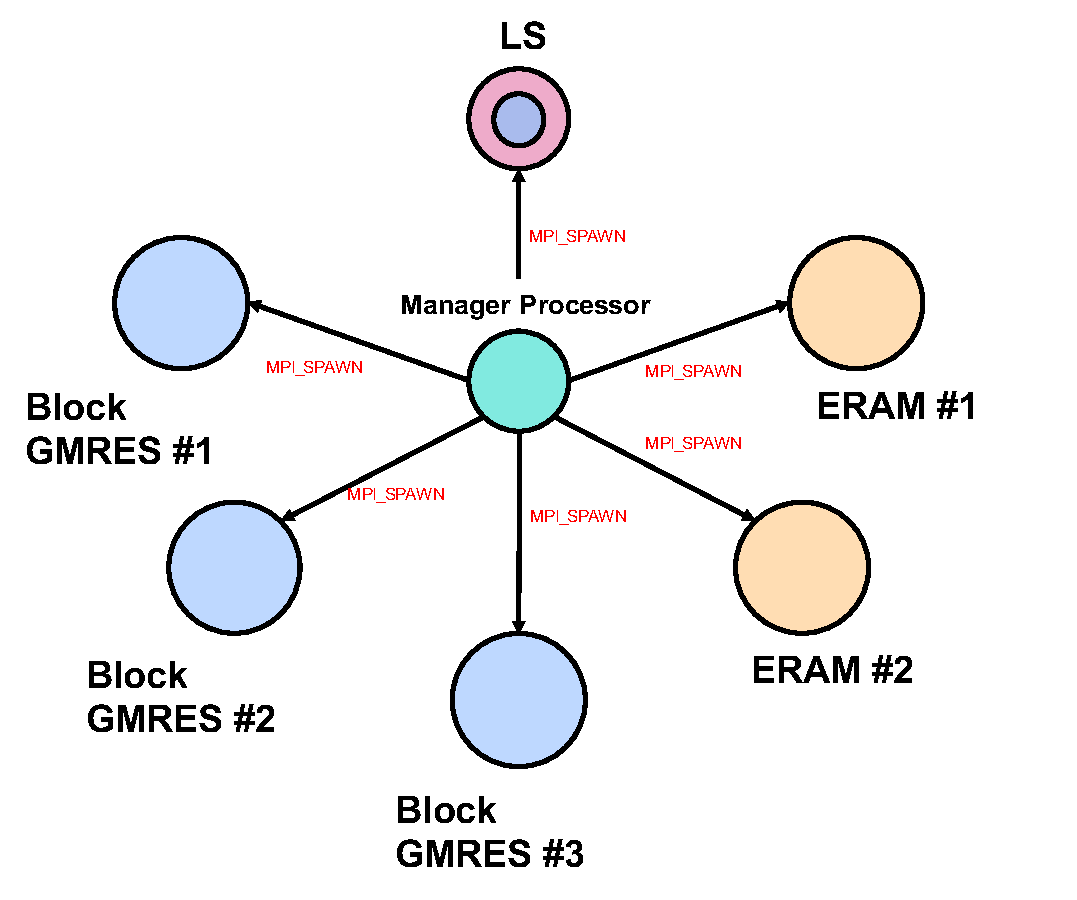
\includegraphics[width=4.8in]{fig/ucmgle.pdf}
	\caption{Manager Engine Implementation for $m$-UCGLE.}
	\label{fig:ucmgle}
\end{figure}

Table \ref{memory} gives the comparison of memory and communication complexity of SpGEMM operation inside $m$-UCGLE and BGMRES with the same number of RHSs. The factors $n$, $nnz$, $s$, $P_g$ and $n_g$ represent respectively the matrix size, the number of non-zero entries of matrix, the number of multiple RHSs, the total number of computing units for BGMRES Components, and the number of BGMRES Components allocated by the manager engine of $m$-UCGLE. The average memory requirement for BGMRES on each computing unit is $\mathcal{O}(\frac{nnz(1+s)}{P_{g}})$. For $m$-UCGLE, the matrix is duplicated $n_g$ times into different allocated linear solvers. Thus the required memory to store the matrix should be scaled with the factor $n_g$ comparing with BGMRES. Due to the localization of computation inside $m$-UCGLE, the total number global communication can be reduced with a factor $\frac{1}{n_g}$ comparing with BGMRES. In practice, the selection of the number to allocate the BGMRES Components should make a balance between the increase of memory requirement and the reduction of global communication.

\begin{table}[htbp]
	\renewcommand{\arraystretch}{1.4}
	\small	
	\caption{Memory and Communication Complexity Comparison between $m$-UCGLE and BGMRES.}
	\label{memory}
	\centering
	\begin{tabular}{c|c|c|c}
		\toprule
		& $m$-UCGLE & BGMRES & ratio  \\
		\midrule
		Memory  &$\mathcal{O}(\frac{nnz(n_g+s)}{P_{g}})$& $\mathcal{O}(\frac{nnz(1+s)}{P_{g}})$ & $\frac{n_g+s}{1+s}$\\
		\midrule
		Communication & $\mathcal{O}(\frac{nnzsP_g}{n_g})$ & $\mathcal{O}(nnzsP_g)$ & $\frac{1}{n_g}$   \\
		\bottomrule
	\end{tabular}
\end{table}

\begin{algorithm}[h]
	\label{skspc}
	\begin{algorithmic}[1]
		\caption{$s$-KS Component}   
		\Function{$s$-KS-EXEC}{$input$: $A, m_a, \nu, r, \epsilon_a$}
		\While{exit==False}
		\State $s$-KS($A, r, m_a, \nu,\epsilon_a$, $output$: $\Lambda_r$)
		\State Send ($\Lambda_r$) to LS
		\If{Recv ($exit==TRUE$)} 
		\State Send ($exit$) to LS Component  \State stop \EndIf
		\EndWhile
		\EndFunction
	\end{algorithmic}  
\end{algorithm}

Here we present in detail the workflow of this new engine. In the beginning, the manager will simultaneously allocate the required number of three kinds of computing components. For each BGMRES[$k$], it will load a full matrix $A$ and its related subgroup $B_k$, and then start to solve Equation (\ref{eq_sub}) separately. Meanwhile, each $s$-KS[$q$] load a full matrix $A$ from local, and start to find the required part of eigenvalues of $A$, through the $s$-KS method, using different parameters such as the shift value $\sigma_q$, the Krylov subspace size $(m_a)_q$, etc. If the eigenvalues of the required number are approximated on $s$-KS[$q$], these values will be asynchronously sent to the manager process. The manager process will always check if new eigenvalues are available from different $s$-KS Components, if yes, it will collect and update the new coming eigenvalues together and send them to B-LSP Component. B-LSP Component will use all the eigenvalues received from manager process to do the pre-treatment of the B-LSP, the parameters gotten will be sent back to the manager process. Immediately, these parameters will be distributed to BGMRES[$k$]. BGMRES[$k$] can use the B-LSP residual constructed by these parameters to speed up the convergence. If the exit signals from all BGMRES Components are received by manager process, it will send a signal to all other components to terminate their executions.

The allocation of a different number of computing components is implemented with MPI\_SPAWN, and their asynchronous communication is assured by the MPI non-blocking sending and receiving operations between the manager process and each computing components.

\begin{algorithm}[h]
	\label{blspc}
	\caption{B-LSP Component}   
	\begin{algorithmic}[1]
		\Function{B-LSP-EXEC}{$input$: $A,b, d$}
		\If {Recv($\Lambda_r$)}
		\State LS{($input$: $A,b,d,\Lambda_r$, $output$: $A_d, B_d, \Delta_d, H_d$)}
		\State Send ($A_d, B_d, \Delta_d, H_d$) to GMRES Component
		\EndIf
		\If{Recv ($exit==TRUE$)} 
		\State stop \EndIf
		\EndFunction
		
	\end{algorithmic}  
\end{algorithm}

\begin{algorithm}[h]
	\label{bgmresc}
	\caption{BGMRES Component}   
	\begin{algorithmic}[1]
		\Function {BGMRES-EXEC}{$input$: $A, m_g, X_0, B, \epsilon_g, L, l$, $output$: $X_m$}
		\State $count=0$
		\State BGMRES{($input$: $A, m, X_0,B$, $output$: $X_m$)}
		\If{$||B-AX_m||<\epsilon_g$}
		\State \Return $X_m$
		\State Send ($exit==TRUE$) to manager process
		\State Stop
		\Else \If{$count \mid L$}
		\If{recv ($A_d, B_d, \Delta_d, H_d$)}
		\State LSUpdateResidual($input$:$A, B, A_d, B_d, \Delta_d, H_d$)
		\State $count++$
		\EndIf
		\Else
		\State set $X_0=X_m$
		\State $count++$
		\EndIf
		\EndIf
		\If{Recv ($exit==TRUE$)} 
		\State stop \EndIf
		\EndFunction
	\end{algorithmic}  
\end{algorithm}

\begin{algorithm}[htbp]
	\caption{Manger of $m$-UCGLE with MPI Spawn}   
	\label{alg:ucmgle}   
	\begin{algorithmic}[1]
		\Function{Master}{$Input: n_g, n_a$}
		\For {$i = 1:n_g$}
		\State MPI\_Spawn executable BGMRES-EXEC[$i$]
		\EndFor
		\For {$j = 1:n_k$}
		\State MPI\_Spawn executable $s$-KS-EXEC[$j$]
		\EndFor
		\State MPI\_Spawn executable B-LSP-EXEC
		\For {$j = 1:n_k$}
		\If{Recv $array[j]$ from $s$-KS-EXEC[$j$]}
		\State Add $array[j]$ to $Array$
		\EndIf
		\EndFor
		\If{$Array \neq NULL$}
		\State Send $Array$ to B-LSP-EXEC
		\EndIf
		\If{Recv $LSArray$ from B-LSP-EXEC}
		\For{$i = 1:n_g$}
		\State Send $LSArray$ to BGMRES-EXEC[$i$]
		\EndFor
		\EndIf
		\For{$i = 1:n_k$}
		\If {Recv  $flag[i]$ for BGMRES-EXEC[$i$]}
		\If{ $flag[i] == exit$}
		\State $flag ^= true$
		\Else
		\State $flag ^= false$
		\EndIf
		\EndIf
		\EndFor
		\If{$flag == true$}
		\State Kill B-LSP-EXEC
		\For {$i = 1:n_g$}
		\State Kill BGMRES-EXEC[$i$]
		\EndFor
		\For {$j = 1:n_k$}
		\State Kill $s$-KS-EXEC[$j$]
		\EndFor
		\EndIf
		\EndFunction
		
	\end{algorithmic}  
\end{algorithm}


Same as UCGLE, $m$-UCGLE has multiple levels of parallelism for distributed memory systems:

\begin{enumerate}
	\item Coarse Grain/Component level: it allows the distribution of different numerical components, including the preconditioning part (B-LSP and $s$-KS) and the solving part (BGMRES) on different platforms or processors;
	\item Medium Grain/Intra-component level, BGMRES and $s$-KS components are both deployed in parallel;
	\item Fine Grain/Thread parallelism for shared memory: the OpenMP thread-level parallelism, or the accelerator level parallelism if GPUs or other accelerators are available.
\end{enumerate} 

\subsection{$m$-UCGLE Implementation on Multi-GPU}

\textcolor{red}{TO DO}

\subsection{Parallel and Numerical Performance Evaluation}

In this section, we evaluate the numerical performance of $m$-UCGLE for solving non-Hermitian linear systems compared with conventional BGMRES.

\subsubsection{Hardware/Software Settings  and Test Sparse Matrices}\label{hardware}

After the implementation of $m$-UCGLE, we test it on the supercomputer with selected test matrices. The purpose of this section is to give the details about the hardware/software settings and test sparse matrices.

\begin{figure*}[htbp]
	\centering
	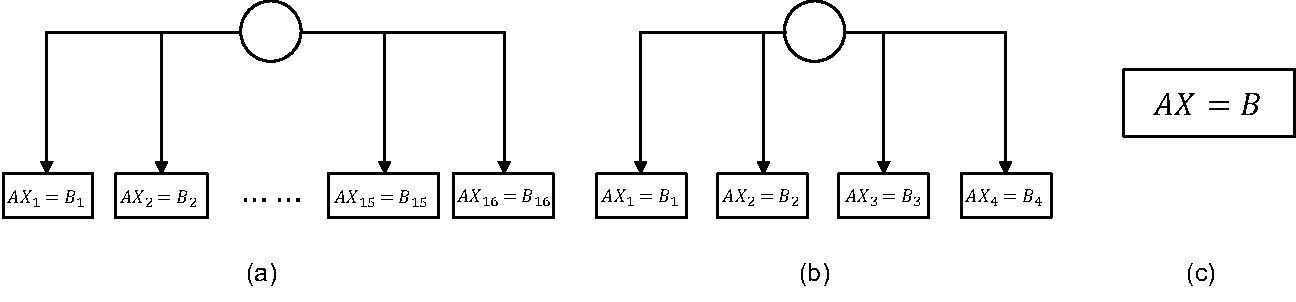
\includegraphics[width=6.4in]{fig/alloc.pdf}
	\caption{Different strategies to divide the linear systems with 64 RHSs into subsets: (a) divide the 64 RHSs into to $16$ different components of $m$-UCGLE, each holds $4$ RHSs; (b) divide the 64 RHSs into to $4$ different components of $m$-UCGLE, each holds $16$ RHSs; (c) One classic BGMRES to solve the linear systems with 64 RHSs simultaneously.}
	\label{fig:alloc}
\end{figure*}

Experiments were obtained on the supercomputer \textit{ROMEO}\footnote{https://romeo.univ-reims.fr}, a system located at University of Reims Champagne-Ardenne, France. Made by Atos, this cluster relies on totally 115 the Bull Sequana X1125 hybrid servers, powered by the Xeon Gold 6132 (products formerly Skylake) and NVidia P100 cards. Each dense Bull Sequana X1125 server accommodates 2 Xeon Scalable Processors Gold bi-socket nodes, and 4 NVidia P100 cards connected with NVLink. In total, this supercomputer includes 3,220 Xeon cores and 280 Nvidia P100 accelerators.

The MPI (Message Passing Interface) used is the OpenMPI 3.1.2, all the shared libraries and binaries were compiled by $gcc$ (version 6.3.0). The released scientific computational libraries Trilinos (version 12.12.1) and LAPACK (version 3.8.0) were also compiled and used for the implementation of $m$-UCGLE. 

\subsubsection{Specific Experimental Setup}

\begin{table}[htbp]
	\renewcommand{\arraystretch}{1.4}
	\small	
	\caption{Alternative methods for experiments, and the related number of allocated component, Rhs number per component and preconditioners.}
	\label{allocname}
	\centering
	\begin{tabular}{c|c|c|c}
		\toprule
		Method & Component nb & RHS nb per component & Preconditioner  \\
		\midrule
		BGMRES(64)  &1& 64 & None\\
		$m$-BGMRES(16)$\times 4$ &4 & 16 & None  \\
		$m$-BGMRES(4)$\times 16$ & 16 & 4 & None   \\
		$m$-UCGLE(16)$\times 4$ & 4 & 16 & B-LSP   \\
		$m$-UCGLE(4)$\times 16$ & 16 & 4 & B-LSP  \\
		\bottomrule
	\end{tabular}
	\label{name}
\end{table}

In the experiments, the total number of RHSs of linear systems to be solved for each test is fixed as $64$. As shown in Figure \ref{fig:alloc}, we propose three strategies to divide these systems into various subgroup: 

\begin{enumerate}
	\item 1 group with all $64$ RHSs solved by classic BGMRES (shown by Figure \ref{fig:alloc}(c));
	\item  $4$ allocated BGMRES Components in $m$-UCGLE with each holding $16$ Rhs (shown by Figure \ref{fig:alloc}(a));
	\item $16$ allocated BGMRES Components in $m$-UCGLE with each holding $4$ Rhs (shown in Figure \ref{fig:alloc}(b)).
\end{enumerate}

Moreover, for $m$-UCGLE with $4$ or $16$ allocated components, they can be applied either with or without the preconditioning of B-LSP using approximate eigenvalues. Denote the special variant of $m$-UCGLE without B-LSP preconditioning as $m$-BGMRES. $m$-BGMRES is also able to reduce the global communications through allocating multiple BGMRES components by the manager engine. Table \ref{name} gives the naming of the five alternatives to solve linear systems with $64$ RHSs and the numbers of their allocated components and the numbers of RHSs per component.

\begin{sidewaystable} % <-- HERE
	\footnotesize
	\caption{Iteration steps of convergence comparison (SMG2S generation suite SMG2S($1,3,4, spec$), relative tolerance for convergence test = $1.0\times10^{-8})$, Krylov subspace size $m_g = 40$, $s_{use} = 10$, $d=15$, $L = 1$, $dnc$ = do not converge in $5000$ iteration steps).}
	\centering
	\renewcommand{\arraystretch}{1.6}
	\begin{tabular}{c*{6}{c}}
		\toprule
		Method            & $spec$ & $m$-BGMRES(4)$\times 16$  & $m$-UCGLE(4)$\times 16$   &  $m$-BGMRES(16)$\times 4$ &  $m$-UCGLE(16)$\times 4$ &  BGMRES(64) \\
		\hline
		TEST-1 &(rand(21.0, 66.0), rand(-21.0,24.0))& \cellcolor{blue!20}239 & 160 & 102 & \cellcolor{red!20}51 & \cellcolor{red!20}51\\
		TEST-2   &   (rand(0.5, 3.0), rand(-0.5,2.0))      &\cellcolor{blue!20}$dnc$  & 176 & 187 & \cellcolor{red!20}62 & 78 \\
		TEST-3    &     (rand(0.2, 5.2), rand(-2.5,2.5))    & \cellcolor{blue!20}$dnc$  & 310 & \cellcolor{blue!20}$dnc$  & \cellcolor{red!20}81 &657 \\
		TEST-4    & (rand(-5.2, -0.2), rand(-2.5,2.5))  & \cellcolor{blue!20}$dnc$  & 320 & 629 & \cellcolor{red!20}99 & 942\\
		TEST-5    &  (rand(-0.23, -0.03), rand(-0.2,0.2))  &\cellcolor{blue!20} 600 & 235 & 170 &\cellcolor{red!20} 99 & 270 \\
		TEST-6    &  (rand(-9.3, -3.2), rand(-2.1,2.1))  & 80 & \cellcolor{blue!20}160 & 85 & 51 & \cellcolor{red!20}38 \\
		\hline
	\end{tabular}
	
	\vspace{5\baselineskip}
	
	\label{time}
	\caption{Consumption time (s) comparison on CPUs (SMG2S generation suite SMG2S($1,3,4, spec$), the size of matrices = $1.792 \times 10^6$, relative tolerance for convergence test = $1.0\times10^{-8})$, Krylov subspace size $m_g = 40$, $l = 10$, $d=15$, $L = 1$, $dnc$ = do not converge in $5000$ iteration steps).}
	\centering
	\renewcommand{\arraystretch}{1.6}
	\begin{tabular}{c*{6}{c}}
		\toprule
		Method            & $spec$ & $m$-BGMRES(4)$\times 16$  & $m$-UCGLE(4)$\times 16$   &  $m$-BGMRES(16)$\times 4$ &  $m$-UCGLE(16)$\times 4$ &  BGMRES(64) \\
		\hline
		TEST-1 &(rand(21.0, 66.0), rand(-21.0,24.0))& \cellcolor{red!20}34.2&	35.3	&133.9	&98.9	&\cellcolor{blue!20}362.8\\
		TEST-2   &   (rand(0.5, 3.0), rand(-0.5,2.0))      & $dnc$  & \cellcolor{red!20}40.9	&231.3	&111.5	&\cellcolor{blue!20}580.6\\
		TEST-3    &     (rand(0.2, 5.2), rand(-2.5,2.5))    & $dnc$  & \cellcolor{red!20}66.0 & $dnc$  & 145.8 & \cellcolor{blue!20}522.5 \\
		TEST-4    & (rand(-5.2, -0.2), rand(-2.5,2.5))  & $dnc$  & \cellcolor{red!20}68.2 & 768.3 & 178.2 & \cellcolor{blue!20}6829.3\\
		TEST-5    &  (rand(-0.23, -0.03), rand(-0.2,0.2))  & 132.3 & \cellcolor{red!20}50.1 & 209.4 & 120.5 & \cellcolor{blue!20}1959.5 \\
		TEST-6    &  (rand(-9.3, -3.2), rand(-2.1,2.1))  & \cellcolor{red!20}11.4 & 34.1 & 87.8 & 91.7 & \cellcolor{blue!20}275.8\\
		\hline
	\end{tabular}
	\label{times}
	
\end{sidewaystable} % <-- HERE


These $64$ RHSs for the tests are all generated in random with different given seed states. All the test matrices from TEST-1 to TEST-6 in Table \ref{convstep} are generated by SMG2S($1,3,4,spec$), the definition of $spec$ functions for different tests are shown in Table  \ref{convstep}. For example, the $spec$ of TEST-1 is given as (rand(21.0, 66.0), rand(-21.0,24.0)), the first part rand(21.0, 66.0) defines that the real parts of given eigenvalues for TEST-1 are the floating numbers generated randomly in the fixed interval [21.0, 66.0], similarly its imaginary parts are randomly generated in the fixed interval [-21.0, 24.0]. The relative tolerance for the convergence test is fixed as $1.0 \times 10^{-8}$, the Krylov subspace size $m_g$ is given as $40$ for all tests, the number of times that B-LSP applied in $m$-UCGLE $l$, the degree of Least Squares polynomial in B-LSP, the number of BGMRES restarts between two times of B-LSP preconditioning are respectively set as $10$, $15$ and $1$.  For $m$-BGMRES(16)$\times 4$, $m$-BGMRES(4)$\times 16$,  $m$-UCGLE(16)$\times 4$ and $m$-UCGLE(16)$\times 4$, their iteration steps in Table \ref{convstep} are defined as the maximal ones among their allocated components to solve the systems. 

\subsubsection{Convergence Result Analysis}

The iteration steps of different methods for convergence are shown in Table \ref{convstep} ($dnc$ in this table significates \textit{do not converge in 5000 iteration steps}). In this table, the blue and red cells represent respectively the worst and the best cases for each test. From Table \ref{convstep}, firstly we can conclude that the enlargement of the Krylov subspace by more RHSs in BGMRES is effective to accelerate the convergence for TEST-1, TEST-2, TEST-3, and TEST-6. However, this acceleration cannot always be guaranteed. Referring to TEST-4 and TEST-5, $m$-BGMRES(16))$\times4$ converge faster than BGMRES(64). Secondly, $m$-UCGLE components converge much faster than their related $m$-BGMRES with the same number of RHSs, except in TEST-6. In the TEST-2, TEST-3, TEST-4, and TEST-5 of this table, $m$-UCGLE with $16$ RHSs works even much better than BGMRES with $64$ RHSs. An extreme special case in TEST-4 shows that convergence of $m$-UCGLE(4)$\times16$ and $m$-UCGLE(16)$\times4$ have the speedup respectively $3\times$ and $9.5 \times$ over $m$-BGMRES(16).  

In conclusion, for most tests, the method that converges the fastest is $m$-UCGLE(16)$\times4$. The combination of enlarging the search space by enough number of RHSs and preconditioning by B-LSP makes substantial acceleration on the convergence of solving linear systems. Moreover, compared with classic BGMRES, due to the preconditioning of B-LSP, $m$-UCGLE with less RHSs and smaller search space can still have a better acceleration of the convergence. The potential damages caused by the localization of computation and reduction of global communications with less RHSs of each component in $m$-UCGLE can be covered by the B-LSP preconditioning.

\subsubsection{Strong Scalability Evaluation}

The iteration step for convergence is not the only concern about the iterative methods. After the convergence comparison of $m$-UCGLE and BGMRES, in this section, we evaluate its strong scalability and performance on supercomputer \textit{ROMEO}.

One important concern of BGMRES is the time cost per iteration, due to the communication bound of SpGEMM. In order to evaluate the parallel performance of $m$-UCGLE on large clusters, we compare the strong scaling of $m$-BGMRES(4)$\times 16$, $m$-UCGLE(4)$\times 16$, $m$-BGMRES(16)$\times 4$, $m$-UCGLE(16)$\times 4$ and BGMRES(64) by their average time cost per iteration. 

\begin{figure}[htbp]
	\centering
	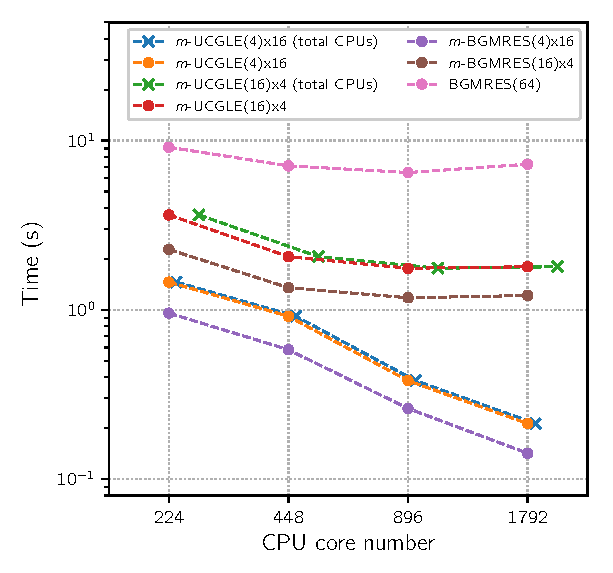
\includegraphics[width=.62\linewidth]{fig/scalable_mucgle.eps}
	\caption{Strong scalability test on CPUs of solving time per iteration for $m$-BGMRES(4)$\times 16$, $m$-UCGLE(4)$\times 16$, $m$-BGMRES(16)$\times 4$, $m$-UCGLE(16)$\times 4$, BGMRES(64); test matrix size is $1.792 \times 10^6$; X-axis refers to the total number of CPUs from 224 to 1792; Y-axis refers to the average execution time per iteration. A base 2 logarithmic scale is used for all X-axis, and a base 10 logarithmic scale is used for all Y-axis.}
	\label{fig_1_case}
\end{figure}

For the strong scaling evaluation on CPUs, the methods tested are set up the same as in Section \ref{convergence}. The test matrix is generated by SMG2S($1,3,4,spec$) with size fixed as $1.792 \times 10^6$. No larger matrices are tested, due to the memory limitation during the Arnoldi projection of BGMRES. The Krylov subspace size $m_g$ for all methods is set as $40$. The average time cost for these methods is computed by 100 iterations. Time per iteration is suitable for demonstrating scaling behavior. The total CPU core number for B-GMRES(64) and all BGMRES Components in $m$-UCGLE and $m$-BGMRES ranges from 224 to 1792. Thus for each BGMRES Component of $m$-BGMRES(4)$\times 16$ and $m$-UCGLE(4)$\times 16$, the number ranges from 14 to 112. Similarly, for each BGMRES Component of $m$-BGMRES(16)$\times 4$ and $m$-UCGLE(16)$\times 4$, this number ranges from 56 to 448. All the tests allocate only 1 $s$-KS Component which always has the same number of CPU cores with each BGMRES Component inside $m$-UCGLE.

In Figure \ref{fig_1_case}, we can conclude that the strong scaling of $m$-BGMRES(4)$\times 16$ and $m$-UCGLE(4)$\times 16$ perform very well, the strong scalability of the rest are bad, especially BGMRES(64). In the beginning, the scalability of $m$-BGMRES(16)$\times 4$ and $m$-UCGLE(16)$\times 4$ is good, but it turns bad quickly with the increase of CPU number. It is demonstrated that the properties of m-UCGLE to promote the asynchronous communication and localize of computation can improve significantly the parallel performance of BGMRES for solving systems with multiple RHSs. Additionally,  for the $m$-BGMRES and $m$-UCGLE with the same number of RHSs, the time per iteration of former is a little less the latter, since $m$-UCGLE introduces the iterative operations (SpGEMM) by B-LSP preconditioning.

Since $m$-UCGLE uses additional computing units for other components especially $s$-KS Component, it is unfair only to compare the scaling performance that total CPU number of all BGMRES Components in $m$-UCGLE equals to these numbers of $m$-GMRES and BGMRES(64). Thus we plot two more curves of $m$-UCGLE(4)$\times 16$ and $m$-UCGLE(16)$\times 14$ with all their CPU numbers (including the CPU of $s$-KS Component) in Figure \ref{fig_1_case}. The two additional curves are respectively the blue and green ones with the marker set as the cross. It is shown that $m$-UCGLE(4)$\times 16$ and $m$-UCGLE(16)$\times 4$ can still have respectively up to $35\times$ and $4 \times$ speedup per iteration against BGMRES(64).


\subsubsection{Time Consumption Evaluation}

After the evaluation of parallel performance, we compare the time consumption of all methods to solve large-scale linear systems with multiple RHSs on CPUs. The test matrices are generated by SMG2S($1,3,4, spec$), the same as the convergence evaluation in Section \ref{convergence}. The size of matrices are all $1.792 \times 10^6$ for the experiments on CPUs, the total numbers of CPU cores for different methods (either BGMRES Components in $m$-UCGLE and $m$-GMRES or conventional BGMRES) are respectively fixed as $1792$, and the Krylov subspace size $m_g$ is set as $40$. The results on CPUs is given in Table \ref{times}, where the blue and red cells represent respectively the worst and the best cases for each test.

We can find that for the TEST-2, TEST-3, TEST-4, TEST-4, $m$-UCGLE(4)$\times 16$ take the least time to converge. For TEST-1 and TEST-6, $m$-BGMRES(4)$\times 16$ takes a little less time than $m$-UCGLE(4)$\times 16$ to get the convergence. For an extremely special case TEST-4, $m$-UCGLE(4)$\times 16$ has about $100\times$ speedup in time consumption over BGMRES(64) to solve the linear systems with $64$ RHSs.

\subsubsection{Analysis}

In conclusion, $m$-UCGLE(4)$\times 16$ and $m$-GMRES(4)$\times 16$ with the most decrease of global communications have the best strong scaling performance. $m$-UCGLE cost a little more time per iteration compared with $m$-BGMRES with the same number of RHSs, but this might be made up by its decrease of iterative steps with B-LSP preconditioning. The experiments in this section demonstrate the benefits of $m$-UCGLE to reduce global communication and promote the asynchronization. Two more important points that cannot be concluded from the experiments in this paper are: 

\begin{enumerate}
	\item The increase of memory requirement should be considered when dividing the whole RHSs into subsets;
	\item The number of RHSs per component of $m$-UCGLE to enlarge the search space and the computation time per iteration should be balanced to achieve the best performance.
\end{enumerate}

\section{Conclusions}

\clearemptydoublepage